% !TeX spellcheck = en_US
\section{RBF interpolation}

\subsection{Theory}

Another approach to interpolate data is using \textit{Radial Basis Functions} (\texttt{RBF}). A very good explanation on how they work is given in \cite{RBF} which is shortly summarized below:

 A function $\phi$ for which $\phi(x)=\phi(\left\|x\right\|)$ is true is called \textit{radial}. Now to be able to interpolate, we need to find the interpolation function $s(x)$ which is the same as the given values $p_i$ in all points.

\begin{align}
	s(x_i)=p_i,\quad i=1,2,\dots,n
\end{align}

The RBF interpolation now consists of a linear combination of $\phi(\left\|x-x_i\right\|)$ for a chosen radial function $\phi$ with $n$ constants $\lambda_i$.

\begin{align}
	s(x)&=	\sum_{i=1}^{n}\lambda_i\phi(\left\|x-x_i\right\|) \\
	%
	p_j&=\sum_{i=1}^{n}\lambda_i\phi(\left\|x_j-x_i\right\|),\quad j=1,2,\dots,n
\end{align}

Therefore, this can be written as a linear matrix equation:

\begin{align}
	\begin{bmatrix}
		\phi(\left\|x_1-x_1\right\|) & \phi(\left\|x_2-x_1\right\|) & \dots  & \phi(\left\|x_n-x_1\right\|) \\
		\phi(\left\|x_1-x_2\right\|) & \phi(\left\|x_2-x_2\right\|) & \dots  & \phi(\left\|x_n-x_2\right\|) \\
		\vdots                       & \vdots                       & \ddots & \vdots                       \\
		\phi(\left\|x_1-x_n\right\|) & \phi(\left\|x_2-x_n\right\|) & \dots  & \phi(\left\|x_n-x_n\right\|)
	\end{bmatrix} 
	\begin{bmatrix}
		\lambda_1 \\
		\lambda_2 \\
		\vdots    \\
		\lambda_n
	\end{bmatrix}
	=
	\begin{bmatrix}
		p_1    \\
		p_2    \\
		\vdots \\
		p_n
	\end{bmatrix}
\end{align}
or simply
\begin{align}
	\Phi\lambda=p
\end{align}

with $\Phi$ being a symmetric $n \times n $ matrix as $\left\|x_j-x_i\right\|=\left\|x_i-x_j\right\|$. There are many possibilities for the radial basis function $\phi(r)$. It can be for example linear ($r$), gaussian ($e^{-r^2}$) or multiquadric ($\sqrt{\left(\frac{r}{\epsilon}\right)^2 + 1}$) with $\epsilon$ being a constant that defaults to the approximate average distance between nodes.

As an example, consider the three points $x_1=0$, $x_1=3$ and $x_1=5$ with $p(x_1)=0.2$, $p(x_2)=0.8$ and $p(x_3)=0.1$ and choose a gaussian function for $\phi$ to get the following:
\begin{align}
	\begin{bmatrix}
		\phi(0) & \phi(3)  & \phi(5) \\
		\phi(3) & \phi(0) & \phi(2) \\
		\phi(5) & \phi(2)  & \phi(0)
	\end{bmatrix} 
	\lambda
	=
		\begin{bmatrix}
			1              & \num{1.23e-4} & \num{1.39e-11} \\
			\num{1.23e-4}  & 1             & \num{1.83e-2}  \\
			\num{1.39e-11} & \num{1.83e-2} & 1
		\end{bmatrix} 
	\begin{bmatrix}
\lambda_1 \\
\lambda_2 \\
\lambda_3
\end{bmatrix}
=
\begin{bmatrix}
0.22\\0.8\\0.1
\end{bmatrix}
\end{align}

Solving this linear matrix equation using \texttt{numpy.linalg.solve} gives us the solution for $\lambda$:
\begin{equation}
	\lambda=\begin{bmatrix}
	0.200 \\0.798  \\0.085
	\end{bmatrix}
\end{equation}

Combined we get the following linear combination for the interpolated function $s(x)$ (Figure \ref{fig:rbf-1}):
\begin{equation}\label{eq:rbf}
	s(x)=0.200\phi(\left\|x\right\|)+
		0.798\phi(\left\|x-3\right\|)+
		0.085\phi(\left\|x-5\right\|)
\end{equation}



\begin{figure}[h] % also temporary
	\centering
	\begin{subfigure}[t]{0.5\textwidth}
		\centering
		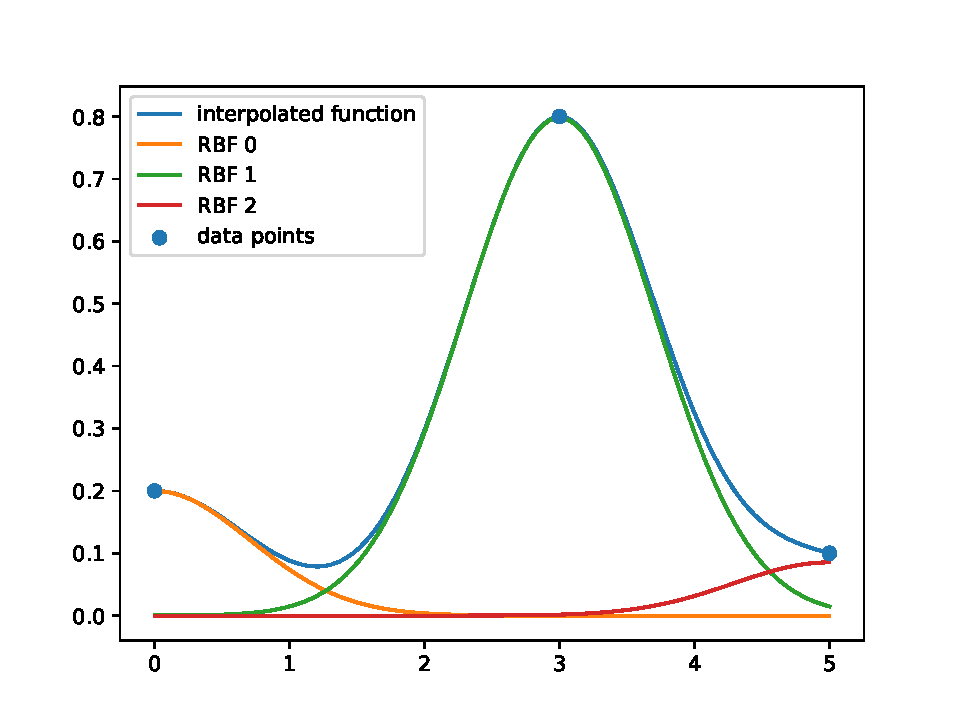
\includegraphics[width=\linewidth]{images/rbf1.pdf}
		\caption{The three functions making up the RBF interpolation from Equation \eqref{eq:rbf}}
		\label{fig:rbf-1}
	\end{subfigure}%
	~ 
	\begin{subfigure}[t]{0.5\textwidth}
		\centering
		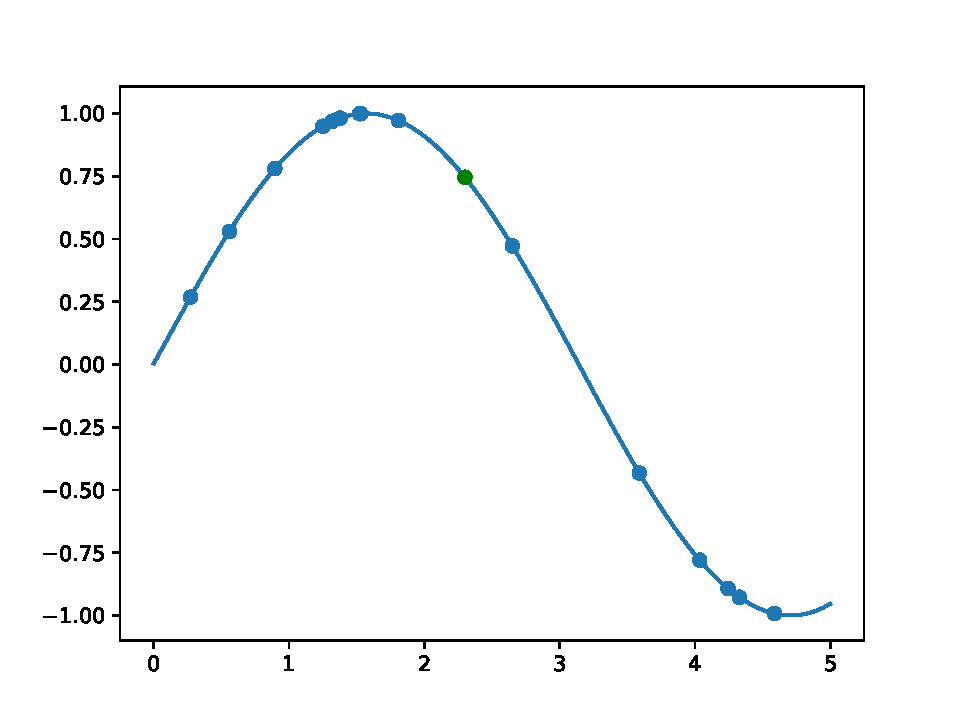
\includegraphics[width=\linewidth]{images/rbf2.pdf}
		\caption{15 points following a sinus-like function with one interpolated value  (\textcolor{Green}{\textbullet})}
		\label{fig:rbf-2}
	\end{subfigure}
	\caption{Two examples for simple RBF interpolation in one dimension}
	
\end{figure}

Applying the same method to a list of random points allows to interpolate their values for arbitrary other points like the green point on the sinus-like curve in Figure \ref{fig:rbf-2}. This can also be trivially extended in $m$ dimensions by replacing $x$ with an $x\in\mathbb{R}^m$ and using a norm in $\mathbb{R}^m$ for $\left\|\ \right\|$.

\subsection{Implementation}

The scipy function \texttt{scipy.interpolate.Rbf} allows directly interpolating a value similar to \texttt{griddata} in Section \ref{sec:griddata-implementation} while using the linear function as the Radial Basis Function ($\phi(r)=r$). A difference in usage is that it only allows interpolating a single value, but as it is pretty quick it is possible to calculate multiple values sequentially.

\subsection{Results}

The results from RBF interpolations can be seen in Figure \ref{fig:rbfresults}. It is far smoother with a gradient from \SIrange{0}{100}{\percent} from the top left to the bottom right corner. Only the lower mass (Figure \ref{fig:rbf1}) has a view outliers. Unlike griddata it is also possible to extrapolate to close values and still get realistic results.

\begin{figure}[h!] % also temporary
	\centering
	\begin{subfigure}[t]{0.5\textwidth}
		\centering
		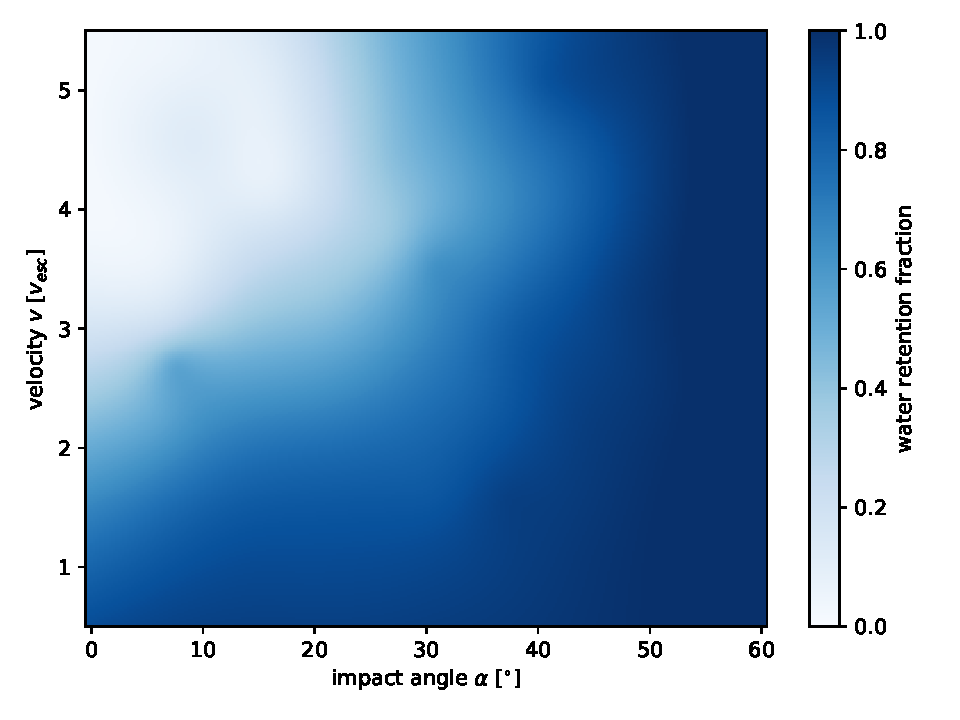
\includegraphics[width=\linewidth]{images/plots/rbf1.pdf}
		\caption{$m_{total}=\num{e22}$, $\gamma=0.6$, $wt=wp=0.15$}
		\label{fig:rbf1}
	\end{subfigure}%
	~ 
	\begin{subfigure}[t]{0.5\textwidth}
		\centering
		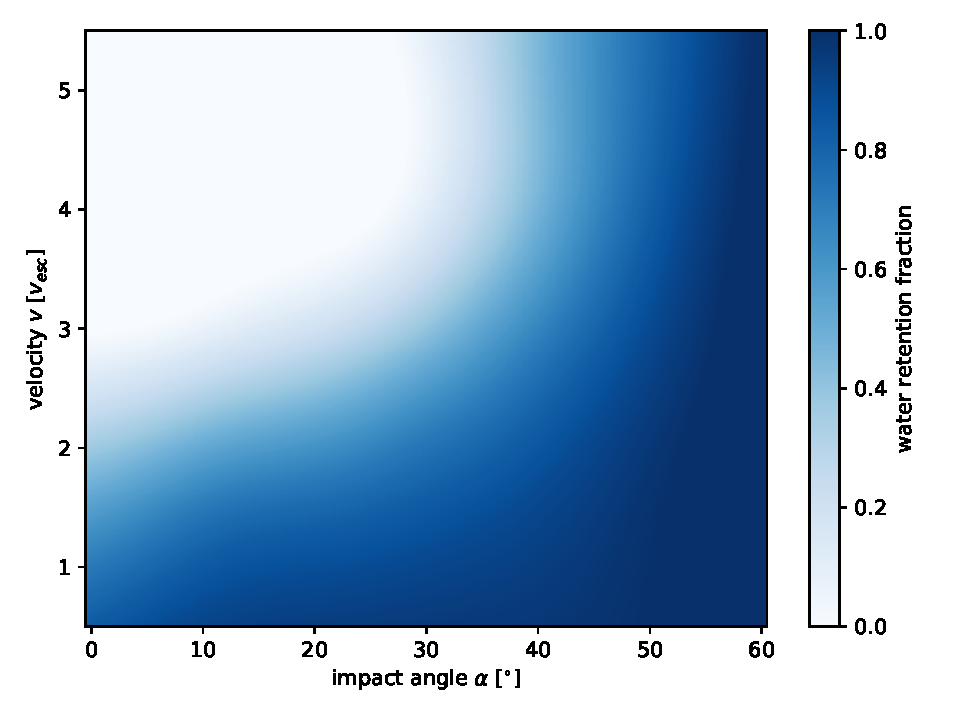
\includegraphics[width=\linewidth]{images/plots/rbf2.pdf}
\caption{$m_{total}=\num{e24}$, $\gamma=0.6$, $wt=wp=0.15$}
		\label{fig:rbf2}
	\end{subfigure}
	\caption{Interpolation result using Radial Basis Functions}
	\label{fig:rbfresults}
\end{figure}
